% =============================================================================
% Architecture globale de l'infrastructure Cloud — TicketManager
% Figure : img/architecture-globale-cloud.png
% =============================================================================

\subsection{Architecture globale de l'infrastructure Cloud}

La plateforme \textit{TicketManager} est déployée sur \textbf{Azure Stack Hub}
dans le groupe de ressources \texttt{AmalBH-RG}. L'infrastructure repose sur
un réseau virtuel segmenté en trois sous-réseaux (administration, base de
données, Kubernetes), provisionné par \textbf{Terraform}. Le
figure~\ref{fig:architecture-globale-cloud} présente l'architecture globale.

\begin{figure}[htbp]
    \centering
    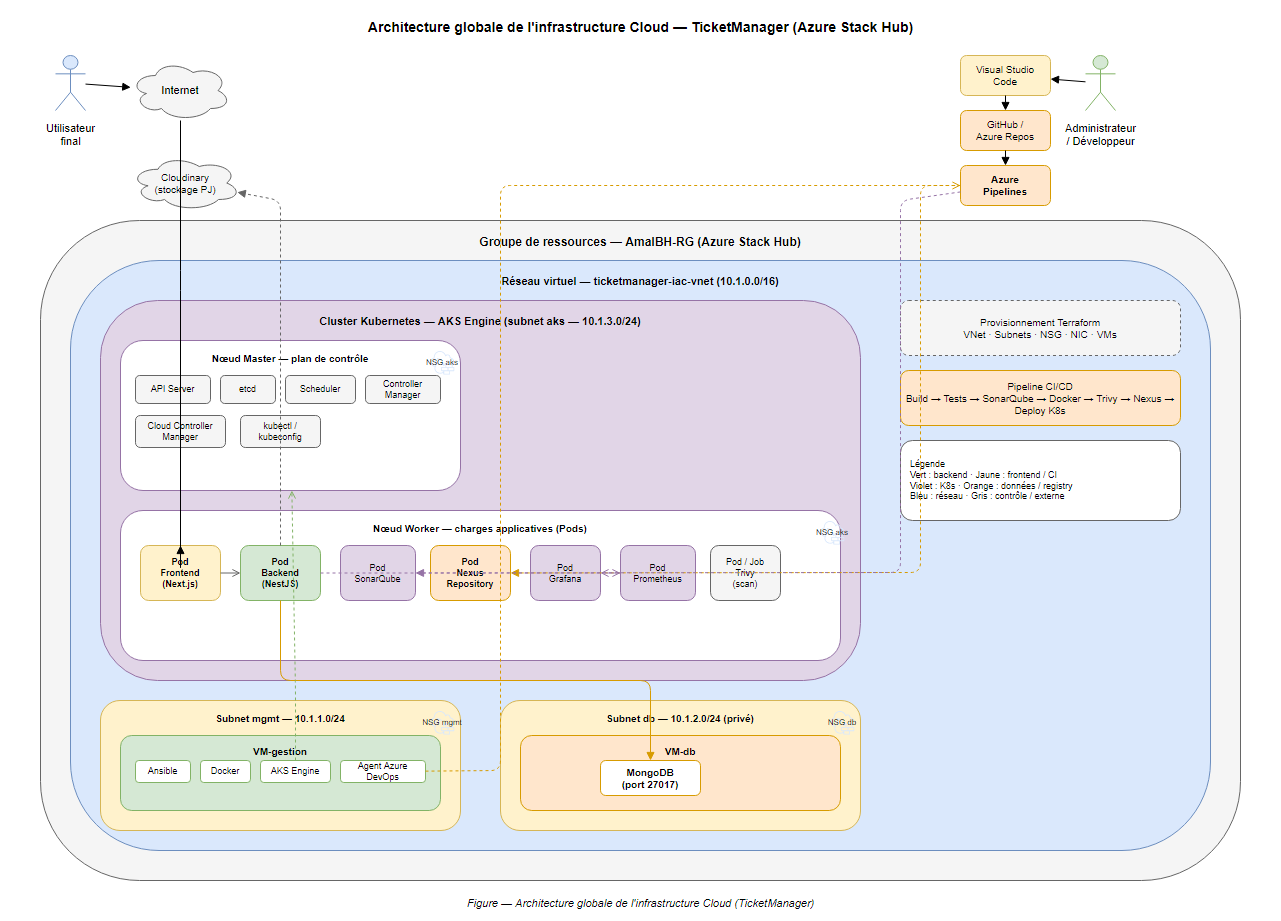
\includegraphics[width=\textwidth]{img/architecture-globale-cloud.png}
    \caption{Architecture globale de l'infrastructure Cloud — TicketManager}
    \label{fig:architecture-globale-cloud}
\end{figure}

\paragraph{Composants principaux.}
\begin{itemize}
    \item \textbf{Cluster Kubernetes} (AKS Engine, subnet \texttt{10.1.3.0/24}) :
          héberge les pods applicatifs (frontend Next.js, backend NestJS) ainsi
          que les services d'industrialisation (SonarQube, Nexus, Grafana,
          Prometheus, Trivy).
    \item \textbf{VM-gestion} (subnet \texttt{10.1.1.0/24}) : administration,
          déploiement du cluster via AKS Engine, agent Azure DevOps et outils
          d'automatisation (Ansible, Docker).
    \item \textbf{VM-db} (subnet \texttt{10.1.2.0/24}, privé) : base de
          données MongoDB, accessible uniquement depuis les sous-réseaux
          administration et Kubernetes.
    \item \textbf{Chaîne CI/CD} : le code source (GitHub / Azure Repos) est
          intégré et déployé via Azure Pipelines ; les images Docker sont
          analysées (Trivy), qualifiées (SonarQube) puis stockées dans Nexus.
    \item \textbf{Services externes} : Cloudinary pour le stockage des pièces
          jointes ; accès utilisateur via Internet au frontend exposé sur le
          cluster.
\end{itemize}
